
In this chapter, we provide evidence to support the claim that our algorithm scales well with increasing amount of computational resources, and that the algorithm is useful, meaning it can provide interesting, non trivial information about the studied model.

\section{Models}

In order to evaluate the algorithm, we first need to define some non-trivial models which we will use to do so. These models, coming from the field of systems biology, are described in this section.

All of the models can be scaled in terms of state and parameter space cardinality by increasing the precision of the piecewise linear approximation.

\subsection{Bi-stable repressilator}

The first model to be considered is the smallest repressilator motif, studied in~\cite{brim2015high,dilao}. It includes two nodes which inhibit each other (see Figure \ref{fig:2Drep} (left)). In biology, this motif is very often present in gene regulatory networks, where $X$ represents product of $gene X$ which inhibits production of $gene Y$ and vice versa.

There are several ways to parametrise this model. In this work, we choose $\phi_X$ and $\phi_Y$ as our parameters, each in the $(0, 1)$ interval (unless explicitly stated otherwise).

\begin{figure}
	\centering
	\begin{center}
		\vspace*{-6mm}
		\hspace*{-1cm}  
		\parbox{4cm}{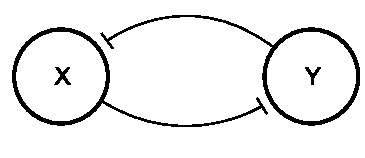
\includegraphics[scale=.6]{2Drep.pdf}}~
		\parbox{6cm}{
			$$\begin{array}{c@{$\,=\,$}l}
			\frac{d[X]}{dt} & k_1 \frac{K_{1}^{n_1}}{K_{1}^{n_1}+[Y]^{n_1}} - \phi_{X}[X]\\[3mm]
			\frac{d[Y]}{dt} & k_2 \frac{K_{2}^{n_2}}{K_{2}^{n_2}+[X]^{n_2}} - \phi_{Y}[Y]
			\end{array}$$
			\center
			$k_1=k_2=1$, $K_{1}=K_{2}=5$, \\
			$n_1=n_2=5$
		}~~
		\vspace*{-5mm}
	\end{center}
	\caption{Bi-stable repressilator regulatory network (left) and its ODE model taken from~\cite{brim2015high} (middle).}
	\vspace*{-0.5em}
	\label{fig:2Drep}
\end{figure}

\subsection{Tri-stable toggle switch}

Tri-stable toggle switch is a model of 3-variable repressilator in which each node inhibits not only one but both of its neighbours (see Figure \ref{fig:3Drep} (left)). Just one of the two ingoing inhibition is enough to repress any entity. Therefore the ODE model possesses multiplication of negative hill function in entity regulation (Fig.~\ref{fig:3Drep} (right)).

Similarly to the bi-stable repressilator, we choose $\phi_X$, $\phi_Y$ and $\phi_Z$ as our parameters, each in the $(0.1, 0.2)$ interval (unless stated otherwise). 

\begin{figure}
	\begin{center}
		% \vspace*{-6mm}
		\hspace*{-1cm}  \parbox{5cm}{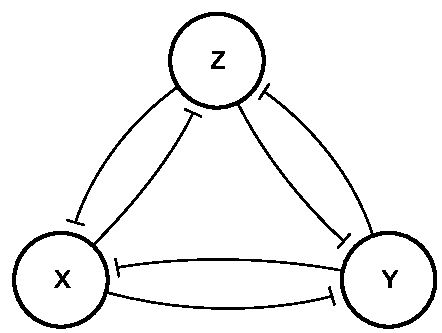
\includegraphics[scale=.6]{triStableRep.pdf}}~
		\parbox{7cm}{
			$$\begin{array}{c@{$\,=\,$}l}
			\frac{d[X]}{dt} & k_{1} \frac{K_{y_1}^{n_1}}{K_{y_1}^{n_1}+[Y]^{n_1}}\cdot \frac{K_{z_1}^{n_2}}{K_{z_1}^{n_2}+[Z]^{n_2}} - \phi_{X}[X]\\[3mm]
			\frac{d[Y]}{dt} & k_{2} \frac{K_{x_2}^{n_3}}{K_{x_2}^{n_3}+[X]^{n_3}} \cdot \frac{K_{z_2}^{n_4}}{K_{z_2}^{n_4}+[Z]^{n_4}} - \phi_{Y}[Y]\\[3mm]
			\frac{d[Z]}{dt} & k_{3} \frac{K_{x_3}^{n_5}}{K_{x_3}^{n_5}+[X]^{n_5}}\cdot \frac{K_{y_3}^{n_6}}{K_{y_3}^{n_6}+[Y]^{n_6}} - \phi_{Z}[Z]
			\end{array}$$
			\center
			$\forall i,j; k_{i}=1$,\\ $K_{x_i}=K_{y_i}=K_{z_i}=5$, 
			$n_j=5$
		}\\
		%\vspace*{-5mm}
	\end{center}
	\caption{Tri-stable toggle switch regulatory network and its ODE model.}
	%\vspace*{-0.5em}
	\label{fig:3Drep}
\end{figure}

\section{Applicability}

To demonstrate the applicability of our approach, we provide an analysis of the stable states of our models, as discovered by the algorithm.

\subsubsection{\textbf{Properties}}

We study two types of stability motifs. First is a terminal strongly connected component, which can be represented using the \ac{HUCTLp} formula $tSCC = \hctlBind{x} \future\ctlA\ctlG \future\ctlE\ctlF x$. Intuitively, a terminal strongly connected component is a maximal set of states that are pairwise reachable (meaning that from any state, I can reach the whole component, but nothing else).

Second motif is a terminal cycle, represented using the formula $tCycle = \hctlBind{x} \future\ctlA\ctlX \future\ctlA\ctlF$. Intuitively, a terminal cycle is a stronger requirement than a terminal component, since the component can contain multiple interleaving cycles, while the terminal cycle property explicitly specifies that there is exactly one cycle (otherwise the $\ctlA$ requirement would be broken).

Notice that we would expect each model to have at least one terminal strongly connected component, however, no such requirement can be imposed to terminal cycles.

In order to show that there are at least two distinct instances of the studied patterns (either $tSCC$ or $tCycle$) in the model, we use the following property: $biPattern = \hctlExists{a \in pattern} pattern \land \neg \future\ctlE\ctlF a$. The property holds in states where the $pattern$ is satisfied and there exists other state (also satisfying $pattern$) not reachable from this state. This is implies presence of two pattern instances, since both our patterns are terminal. Also notice the use of the $exists-in$ operator, which guarantees only appropriate $z$ are considered, thus simplifying the property description and computation performance. 

Such formula can be further generalised to imply presence of three distinct instances: $triPattern = \hctlExists{a \in pattern} \hctlExists{b \in pattern} pattern \land \neg \future\ctlE\ctlF a \land \future\ctlE\ctlF b \land (\hctlAt{a} \future\ctlE\ctlF b)$. 

Finally, we can be interested in presence of exactly one instance (or exactly two) of the studied pattern. To this end, we can simply use the property $single = pattern \land \neg biPattern \land \neg triPattern$. 

\subsubsection{\textbf{Bi-stable repressilator}}

The results of our analysis of the bi-stable repressilator are presented in Figures \ref{fig:biSCC} and \ref{fig:biCycle}. Each figure contains a state space plot and a parameter space plot, where green colour signifies the presence of exactly one pattern instance and the yellow colour signifies presence of exactly two pattern instances. Furthermore, in the state space plot, the mixture of green and yellow represents that either one or two instances of the studied pattern are present, depending on the parameter valuation.

The results of our terminal component analysis are presented in Figure \ref{fig:biSCC}. As expected, the model contains either one or two terminal components, depending on the parameter valuation. Furthermore, the location of these components is clearly visible in the state space plot (right). 

The analysis of the terminal cycles is presented in Figure \ref{fig:biCycle}. As we can see, the model contains parameter valuations for which no terminal cycle is present. For these valuations a manual inspection revealed that multiple non-terminal cycles are present in the model.

\begin{figure}
	
	\begin{center}
		\begin{overpic}[width=.5\textwidth]{results/2D/scc_state.png}\end{overpic}\hfill
		\begin{overpic}[width=.5\textwidth]{results/2D/scc_param.png}\end{overpic}\hfill
	\end{center}
	
	\caption{Presence of two terminal strongly connected components in the bi-stable repressilator model. The parameter space (right) has been zoomed to cover only the interesting area.  }
	\label{fig:biSCC}
\end{figure}

\begin{figure}
	
	\begin{center}
		\begin{overpic}[width=.5\textwidth]{results/2D/cycle_state.png}\end{overpic}\hfill
		\begin{overpic}[width=.5\textwidth]{results/2D/cycle_param.png}\end{overpic}\hfill
	\end{center}
	
	\caption{Presence of two terminal cycles in the bi-stable repressilator model.}
	\label{fig:biCycle}
\end{figure}

\subsubsection{\textbf{Tri-stable toggle switch}}

The results of our analysis of the tri-stable toggle switch are presented in Figures \ref{fig:triSCC} and \ref{fig:triCycle}. The presentation of these results is affected by the dimensionality of the model in question. Mainly, we present the dependence of just two variables (parameters) and project the remaining values into such plane. This makes the colour-mixing approach taken in the previous case infeasible, since there is no way to distinguish truly intersecting properties from the projected ones. Therefore we assume the reader is more interested in higher counts of pattern instances and prioritise those. All visualisations are produced directly using Pithya and the full results are available as a digital attachment to this work. The reader is therefore encouraged to inspect the data directly in case of any further questions.

As we can see in Figure \ref{fig:triSCC}, the model can contain either one, two, or three terminal strongly connected components, depending on the parameter valuations. The state space covered by the components appears to be continuous due to the dimensional projection. In fact, the three components are located in the corners of the projected triangle, while the triangle itself spans all three dimensions. Depending on the parameter valuation, the triangle can contract to produce two, or just one component.

Figure \ref{fig:triCycle} then presents similar results, but as we can see, the stronger requirement of terminal cycles produces smaller result set. Interesting observation is that for the selected parametrisations, at least one terminal cycle is always present (This is not directly implied by the plots, since they are projections. It has been verified separately).

\begin{figure}
	
	\begin{center}
		\begin{overpic}[width=.5\textwidth]{results/3D/scc_state.png}\end{overpic}\hfill
		\begin{overpic}[width=.5\textwidth]{results/3D/scc_param.png}\end{overpic}\hfill
	\end{center}
	
	\caption{Presence of one (green), two (yellow) and three (blue) terminal strongly connected components in the tri-stable toggle switch model. Remaining dimensions have been projected into the plots.  }
	\label{fig:triSCC}
\end{figure}

\begin{figure}
	
	\begin{center}
		\begin{overpic}[width=.5\textwidth]{results/3D/cycle_state.png}\end{overpic}\hfill
		\begin{overpic}[width=.5\textwidth]{results/3D/cycle_param.png}\end{overpic}\hfill
	\end{center}
	
	\caption{Presence of one (green), two (yellow) and three (blue) terminal cycles in the tri-stable toggle switch model. Remaining dimensions have been projected into the plots.}
	\label{fig:triCycle}
\end{figure}

\section{Scalability}

We evaluate the scalability of the algorithm using two \ac{CTL} and two \ac{HUCTLp} properties:

\begin{align*}
	\varphi_1 = \future\ctlE\ctlF center \\
	\varphi_2 = \future\ctlA\ctlF center \\
	\varphi_3 = \hctlBind{x} \future\ctlE\ctlX \future\ctlE\ctlF x \\
	\varphi_4 = \hctlBind{x} \future\ctlA\ctlX \future\ctlA\ctlF x \\
\end{align*}

Here, $center$ specifies a proposition which is satisfied only in the very middle state of the model.

Each property has been tested on a model with an appropriate state space size (since \ac{HUCTLp} properties are usually much harder to verify). The results of this analysis are presented in Table \ref{tab:scale}. As we can see, the algorithm scales with increasing amount of computational resources, the only problem being the $\ctlA\ctlF$ query on the two dimensional model. Further inspection revealed that the algorithm is not able to parallelise this query very well, because the valid state space does not provide much opportunities to branch the exploration into multiple parallel directions.

The evaluation has been performed on a 64-core server and is taken as an overage over five runs. However, the access to this server was not exclusive. The computation was restricted to the specified amount of processors and RAM during each experiment.

\begin{table}[]
	\centering
	\caption{Scalability results}
	\label{tab:scale}
	\begin{tabular}{l|M{0.8cm}M{0.8cm}M{0.8cm}M{0.8cm}|M{0.8cm}M{0.8cm}M{0.8cm}M{0.8cm}N}
		& \multicolumn{4}{l|}{Bi-stable repressilator}         & \multicolumn{4}{l}{Tri-stable toggle switch}        &\\[8pt] \hline
		State count & \multicolumn{2}{c}{$\sim2.25e4$} & \multicolumn{2}{c|}{$\sim$1000} & \multicolumn{2}{c}{$\sim3.4e5$} & \multicolumn{2}{c}{$\sim3000$} &\\[8pt] \hline
		Property    & $\varphi_1$ & $\varphi_2$ & $\varphi_3$ & $\varphi_4$ & $\varphi_1$ & $\varphi_2$ & $\varphi_3$ & $\varphi_4$  &\\[8pt] \hline
		1cpu/4gb    & 112s & 35s & 259s & 89s & 63s & 62s & 125s & 30s &\\[8pt]
		2cpu/8gb    & 76s & 31s & 168s & 71s & 45s & 42s & 86s & 20s  &\\[8pt]
		4cpu/16gb   & 65s & 26s & 110s & 44s & 35s & 36s & 57s & 17s &\\[8pt]
		8cpu/32gb   & 38s & 26s & 65s & 40s & 30s & 28s & 39s & 14s &\\[8pt]
	\end{tabular}
\end{table}
